\linespread{1.5}
O diagrama abaixo mostra um reservatório cilíndrico provido de um furo no fundo.
\begin{figure}[H]
    \centering
    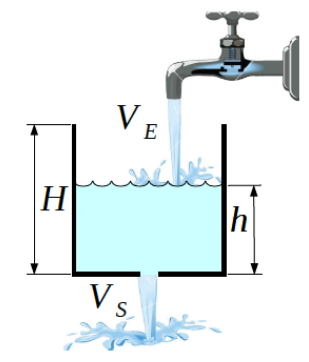
\includegraphics[width=0.3\linewidth]{fig/edo34}
\end{figure}
A água entra no reservatório com uma vazão $V_E$ e sai pelo furo com uma vazão $V_S$. Nessas condições, a altura da água dentro do reservatório, $h(t)$, é solução da quação diferencial de 1ª ordem:
\begin{equation}
    \label{eq:edo341}
    \Dot{h} = \frac{V_E - V_S}{A}
\end{equation}

Sendo $A$ a área da secção horizontal do reservatório. Considerando $V_E$ constante e $V_S$ dada pela fórmula de Torricelli:
\begin{equation}
    \label{eq:342}
    V_S = a\sqrt{2gh}
\end{equation}

sendo $g$ a aceleração da gravidade e $a$ a área do furo. A E.D.O. (\ref{eq:edo341}), portanto, escreve-se como:
\begin{equation}
    \label{eq:edo343}
    \Dot{h} = \frac{V_E - a\sqrt{2gh}}{A}
\end{equation} 
Dadas as informações acimas, pede-se:
\begin{itemize}
    \item[\textbf{a)}] Determine a solução geral da E.D.O. (\ref{eq:edo343});
    \item[\textbf{b)}]Determine a solução particular que satisfaz a condição inicial $h(0) = 0$, ou seja, no instante inicial o reservatório está vazio;
    \item[\textbf{c)}] Faça um esboço do gráfico da solução particular obtida em \textbf{b)};
    \item[\textbf{d)}]Considerando os valores constantes na tabela abaixo, determine qual deve ser altura $H$ do reservatório para que não ocorra transbordamento de água.
    \begin{table}[H]
    \centering
    \begin{tabular}{|c|c|}
    \hline
    \textit{A}     & 1250 $cm^2$      \\ \hline
    \textit{a}     & 0,7 $cm^2$       \\ \hline
    \textit{g}     & 9,8 $m/s^2$      \\ \hline
    \textit{$V_E$} & 12 litros/minuto \\ \hline
    \textit{H}     & ?                \\ \hline
    \end{tabular}
    \end{table}
\end{itemize}